\vfill 

\section*{Fitting a Quadratic Model}

Use \myDesmos to find a \myEmph{quadratic} regression model. 
To do this, use the \myDesmos commands in the table above. 

\myProblemsWithContent
{
    Find the model parameters listed below.
    \begin{center}
        \renewcommand{\arraystretch}{1.4}
        \begin{tabular}{r|l|c}
            model & best fit parameters & $r^2$ or $R^2$ \\ 
            \midrule
            {\itshape Quadratic} 
            & $\bm{a_2} =$ \underline{\hspace{0.5in}} & $R^2 =$ \underline{\hspace{0.5in}} \\
            & $\bm{b_2} =$ \underline{\hspace{0.5in}} & \\
            & $\bm{c_2} =$ \underline{\hspace{0.5in}} & \\
            \end{tabular}
        \end{center}
}
{  
    When $R^2$ is close to zero, it's not a good fit. 
    When $R^2$ is close to one, it is a good fit.
    Compare it to the linear fit. Is this better or worse?
    Explain your thinking \myEmph{as a full sentence}.
}[\small]

\myProblemsWithContent
{
    Sketch a scatterplot of the $(x,y)$ data. 
    Then sketch the parabola $y = \bm{a_2} + \bm{b_2}x + \bm{c_2}x^2$ based on \myDesmos.\newline
        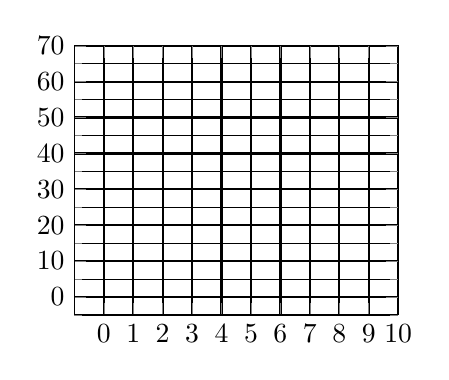
\begin{tikzpicture}
            \begin{axis}[
                scale=0.6,
                grid = both,
                xmin=-1, xmax=10, xtick distance=1, xtickmin=0,
                ymin=-5, ymax=70, ytick distance=10, minor y tick num=1,
                major grid style={solid,thick,black},
                minor grid style={solid,very thin,black},
            ]
            \end{axis}
        \end{tikzpicture}
}
{
    How many points does the parabola go through?
}[\small]